\subsection{Regularized Neural Networks}

\subsubsection{Weight Decay}

\begin{figure}[h!]
  \centering
  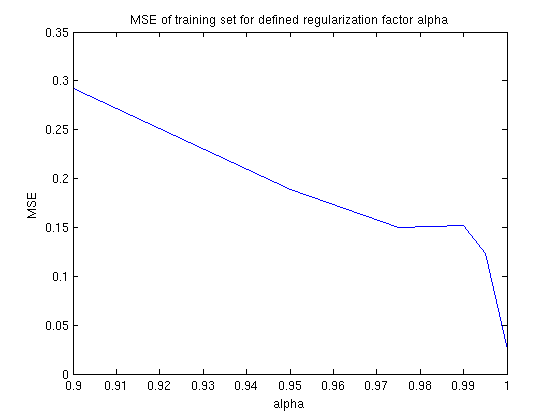
\includegraphics[width=0.75\textwidth]{./figures/3/3_1_mse_train_wd.png}
  \caption{MSE des Trainingssets mit \emph{weight decay} für unterschiedliche $\alpha$}
  \label{fig:3_1_mse_train_wd}
\end{figure}

\begin{figure}[h!]
  \centering
  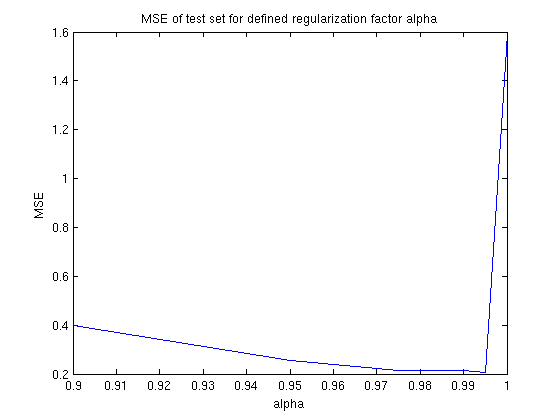
\includegraphics[width=0.75\textwidth]{./figures/3/3_1_mse_test_wd.png}
  \caption{MSE des Testsets mit \emph{weight decay} für unterschiedliche $\alpha$}
  \label{fig:3_1_mse_test_wd}
\end{figure}

Abbildungen \ref{fig:3_1_mse_train_wd} und \ref{fig:3_1_mse_test_wd} zeigen den Fehler des Trainings- bzw. Testsets für unterschiedliche $\alpha$. Bei \emph{weight decay} wird dem MSE ein \emph{penalty term} dazuaddiert, der sich aus den Gewichten berechnet. Dadurch wird bei steigenden Gewichten auch der Fehler größer, was dazu führt, dass Gewichte keine sehr großen Werte annehmen. Dadurch wird verhindert, dass sich die Gewichte zu sehr an die Trainingsdaten anpassen, dadurch wird Overfitting vermindert. Bei kleinem $\alpha$ steigt der Fehler, da die Gewichtssumme zu stark ins Gewicht fällt. Erhöht man $\alpha$, kommt man irgendwann zu dem Wert, bei dem der Fehler minimiert wird, indem die Größe der Gewichte sinnvoll beschränkt wird. Erhöht man dann $\alpha$ weiter, kommt man wieder zum gleichen Ergebnis wie ohne weight decay, nämlich Overfitting.

Bei diesem Beispiel ergab sich der beste Wert zu $\alpha = 0.995$.

\emph{Weight decay} erzielt den gleichen Effekt wie der \emph{regularization term} bei linearer Regression. Bei Betrachtung der Formeln sieht man, dass diese prinzipiell übereinstimmen, nämlich der MSE und die Summe der Gewichte, jeweils wiederum gewichtet.

\begin{figure}[h!]
  \centering
  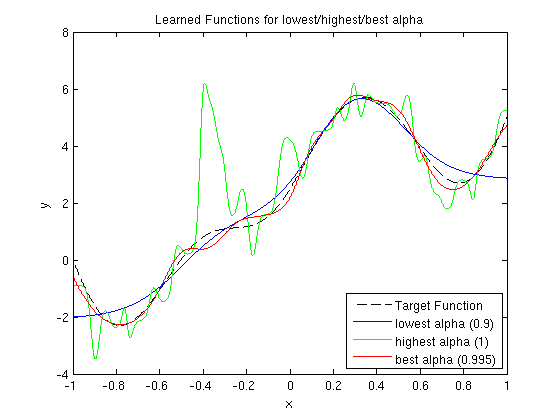
\includegraphics[width=0.75\textwidth]{./figures/3/3_1_learned_wd.png}
  \caption{Gelernte Funktionen mit \emph{weight decay} für das geringste, größte und beste $\alpha$}
  \label{fig:3_1_learned_wd}
\end{figure}

Abbildung~\ref{fig:3_1_learned_wd} zeigt die gelernte Funktion für das geringste, größte und beste $\alpha$. Man erkennt, dass bei zu niedrigem $\alpha$ die Kurve zu ``flach'' ist, da die Gewichte zu stark in den Fehler einfließen. Bei zu hohem $\alpha$ erhält man das gleiche Ergebnis wie ohne weight decay.


\subsubsection{Early Stopping}

\begin{figure}[h!]
  \centering
  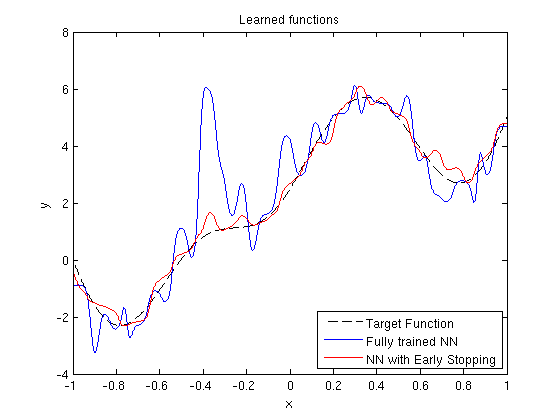
\includegraphics[width=0.75\textwidth]{./figures/3/3_1_learned_es.png}
  \caption{Gelernte Funktionen mit \emph{early stopping} des komplett trainierten Netzwerkes und des Early-Stopped Netzwerkes}
  \label{fig:3_1_learned_es}
\end{figure}

Abbildung \ref{fig:3_1_learned_es} zeigt die gelernte Funktion des komplett trainierten Netzwerkes bzw. des Early-Stopped Netzwerkes. Die gelernte Funktion des komplett trainierten Netzwerkes ist bereits ein vertrautes Bild, sie entspricht der der vorangegangenen Methoden. Beim \emph{early stopping} bricht man den Lernvorgang des Neuronalen Netzwerkes dann ab, wenn der Fehler auf den Testdaten am geringsten ist (also wenn die Gewichte noch ``generell'' genug sind, und es noch nicht zu Overfitting gekommen ist). Dadurch ergibt sich ein sehr geringer Fehler.

Das \textsc{Matlab}-Skript (siehe Anhang) ermittelt den geringsten Fehler auf den Testdaten, und bei welcher Epoche dieser auftritt:

\noindent \texttt{fully trained NN with 40 neurons: 0.028497 mse on training set, 1.572938 mse on testset\\
minimal mse is 0.232383 at epoch 11\\
early stopping trained NN with 40 neurons: 0.137280 mse on training set, 0.232383 mse on testset}


\subsubsection{Comparison}

\paragraph{Different Number of Neurons}

Bei unterschiedlichen Anzahlen von Neuronen treten die genannten Effekte auf: sind die Neuronen zu wenig, kann die geforderte Funktion nur schlecht angenähert werden. Ist die Anzahl der Neuronen zu hoch, kommt es zu Overfitting. Im Beispiel gibt es ein Optimum hinsichtlich der Anzahl der Neuronen, welches bei 6 Neuronen liegt (siehe Abb. \ref{fig:3_mse_test}). Bei den angegebenen Neuronenanzahlen erreicht das NN mit 8 Neuronen den minimalen MSE von ca. 0.21.

\paragraph{Weight Decay}

Für den richtigen Regularisierungsfaktor $\alpha$ wurden bessere Ergebnisse erzielt als mit der vorherigen Methode. Es muss jedoch für jeden möglichen Faktor $\alpha$ das gesamte NN trainiert werden, was sehr zeitaufwändig ist. Durch den Regularisierungsfaktor verhindert man den Overfitting-Effekt. Mit Weight Decay erreicht man einen minimalen MSE von ca. 0.2.

\paragraph{Early Stopping}

Early Stopping erzielt etwas schlechtere Ergebnisse als Weight Decay, dafür muss nur ein NN komplett trainiert werden, und ein weiteres NN nur bis zur optimalen Epoche. Dadurch verringert sich die Rechenzeit drastisch. Mit Early Stopping erreicht man einen minimalen MSE von ca. 0.23.

